\chapter{Esempi di Applicazioni per Hololens 2}\label{chap:capitolo3}

I possibili settori di applicazione di HoloLens 2 sono svariati. In generale, in qualsiasi ambiente la realtà mista può essere introdotta per aumentare produttività, efficienza e sicurezza.

Di seguito vengono riportati alcuni ambiti in cui l'introduzione di HoloLens 2 ha giocato un ruolo fondamentale per quanto riguarda gli aspetti appena descritti.

\section{Ambito Industriale}\label{sec:Sezione3.1}
Per quanto riguarda l'ambito industriale si può fare riferimento ai partner Microsoft, come Airbus.
Airbus è un pioniere nella tecnologia aerospaziale e leader nella progettazione e produzione di aerei commerciali e militari, satelliti e veicoli di lancio, si è impegnata a trasformare i processi industriali tradizionali attraverso l'uso della realtà mista. L'azienda ha stretto una partnership con Microsoft per utilizzare la realtà mista di Azure e HoloLens 2 come mezzo per accelerare la progettazione e la produzione di aeromobili, aumentando al contempo la sicurezza e la funzionalità e garantendo opportunità di sviluppo professionale per i dipendenti. Servizi intelligenti come Azure Remote Rendering stanno cambiando il modo in cui vengono comunicate le idee complesse. La capacità di creare applicazioni multiutente con riconoscimento dello spazio con Azure Spatial Anchors promuove una maggiore collaborazione aumentando la qualità, la sicurezza e la protezione. Airbus sta usando la realtà mista di Azure per sbloccare tutto il potenziale di HoloLens 2 e, di conseguenza, prevede di ridurre i tempi di convalida del progetto dell'80\% e di accelerare le attività complesse durante l'assemblaggio del 30\%.

Airbus ha impiegato 40 anni per costruire i suoi primi 10.000 velivoli. Nei prossimi 20 anni, il gigante aerospaziale mira a costruirne altri 20.000, una sfida formidabile che richiederà innovazioni all'avanguardia.

Jean-Brice Dumont, Executive Vice President of Engineering di Airbus, afferma:

\begin{center}
    “La nostra sfida nei prossimi anni è quella di produrre più velivoli più velocemente, e per questo dobbiamo consentire ai nostri lavoratori di essere molto meglio equipaggiati e di essere molto più efficaci in quello che fanno. Dobbiamo alzare il tiro.
    Per affrontare questa sfida, intendiamo fare un uso intenso della realtà mista ed è per questo che abbiamo stretto una partnership con Microsoft.
    La realtà mista può aiutarci ad aumentare la qualità, la sicurezza e la protezione. Il livello di errore umano è significativamente ridotto e, nel settore aerospaziale, una maggiore qualità è una maggiore sicurezza".
\end{center}

La tecnologia Microsoft Mixed Reality può essere utilizzata per aiutare gli addetti alla produzione di Airbus ad accedere a informazioni e istruzioni mentre hanno le mani occupate, ad esempio. Può anche facilitare la formazione senza impegnare attrezzature costose o persino richiedere al tirocinante di recarsi nel luogo in cui si trova l'attrezzatura. Questo è solo l'inizio: Airbus ha identificato più di 300 casi d'uso per la realtà mista.

Airbus ha ottenuto risultati impressionanti nelle sue prove e implementazioni della tecnologia di realtà mista Microsoft nella formazione, nella progettazione e nella produzione.

La realtà mista consente ai tirocinanti aerospaziali di apprendere in un ambiente virtuale immersivo senza la necessità di un vero aereo fisico o di parti. Questo ambiente 3D può offrire funzionalità che l'allenamento nella vita reale non può offrire, come la possibilità di visualizzare gli elementi in tre dimensioni da qualsiasi angolazione.

HoloLens aiuta i progettisti di Airbus a testare virtualmente i loro progetti per vedere se sono pronti per la produzione. La realtà mista accelera notevolmente il processo, riducendo il tempo impiegato dell'80\%.

La tecnologia della realtà mista può anche aiutare i lavoratori della linea di produzione ad accedere a informazioni cruciali mantenendo le mani libere. Le informazioni digitali, come istruzioni o diagrammi, possono essere sovrapposte a un vero macchinario per aiutare in attività complesse o difficili. Questi tipi di soluzioni di realtà mista hanno consentito ad Airbus di ridurre di un terzo i tempi di produzione migliorando al contempo la qualità.

\section{Ambito Sanitario}\label{sec:Sezione3.2}
In ambito sanitario sono stati prodotti vari articoli scientifici che, grazie ad HoloLens, propongono soluzioni per migliorare la precisione e l'efficienza delle operazioni e per ridurre l'esposizione degli operatori alle radiazioni.

La tecnologia olografica di HoloLens 2 può essere utile per interventi guidati da CT \footnote{La tomografia computerizzata (in inglese computed tomography) è un processo che visualizza le informazioni anatomiche da un piano di sezione trasversale del corpo.} rendendoli più sicuri ed efficienti.
In questo articolo \cite{Augmented-Reality-Assisted-CT-Guided-Interventions} È stato eseguito uno studio prospettico per valutare il direzionamento dell'ago guidato da CT su un fantoccio addominale (Figura \ref{fig:figure3a}) con e senza guida AR (rispettivamente Figura \ref{fig:figure3d} e Figura \ref{fig:figure3c}). 
L'allineamento è stato eseguito automaticamente su una griglia TC utilizzata di routine nella pratica clinica, invece di utilizzare marker esterni basati su immagini, richiesti invece in altri sistemi.

Hanno partecipato in totale otto operatori con diversa esperienza clinica che hanno eseguito un totale di 86 passaggi con ago. L'efficienza della procedura, la dose di radiazioni e i tassi di complicanze sono stati confrontati con e senza guida AR.

In Figura \ref{fig:figure3d} l'allineamento con il mondo reale appare accurato, le linee della griglia CT reali sono allineate con le linee della griglia virtuale. L'ago è allineato con la guida virtuale (linea viola) che mostra la traiettoria ideale verso la lesione selezionata (pallina verde).

\begin{figure}[t]
    \centering
    \begin{subfigure}{0.45\textwidth}
        \centering
        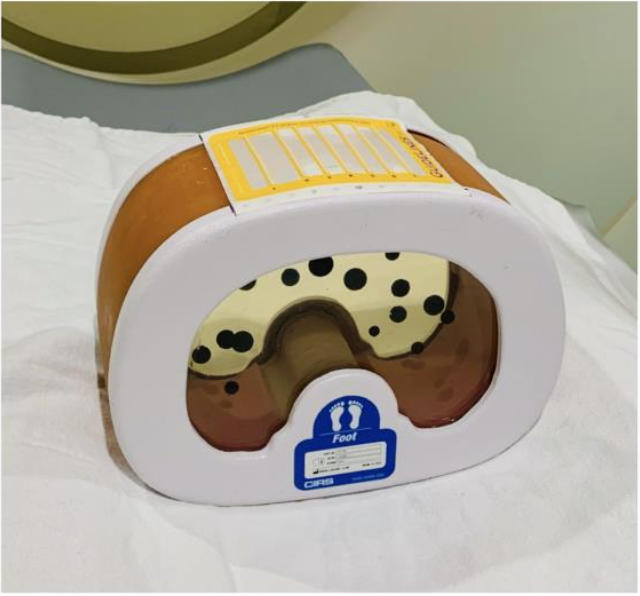
\includegraphics[width=\textwidth]{images/phantom.png}
        \caption{Griglia CT applicata alla superficie del modello.}
        \label{fig:figure3a}
    \end{subfigure}
    \begin{subfigure}{0.45\textwidth}
        \centering
        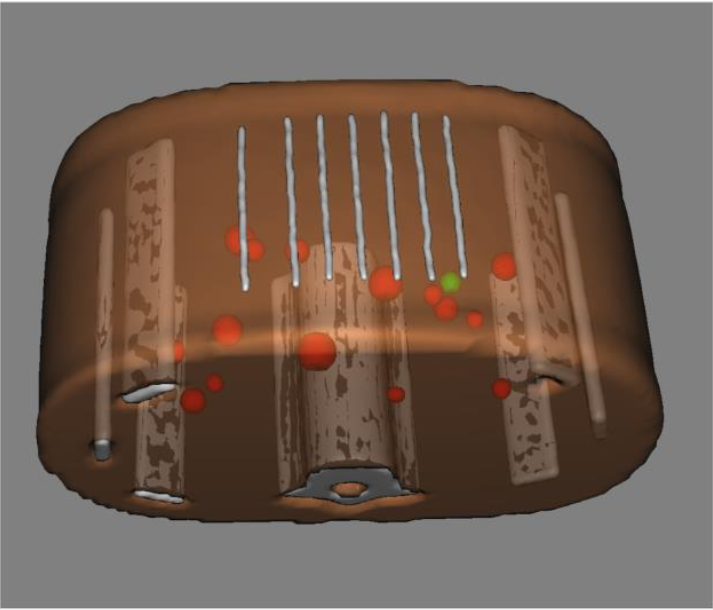
\includegraphics[width=\textwidth]{images/phantom-3D-model.png}
        \caption{Modello 3D del fantoccio.}
        \label{fig:figure3b}
    \end{subfigure}
    \begin{subfigure}{0.45\textwidth}
        \centering
        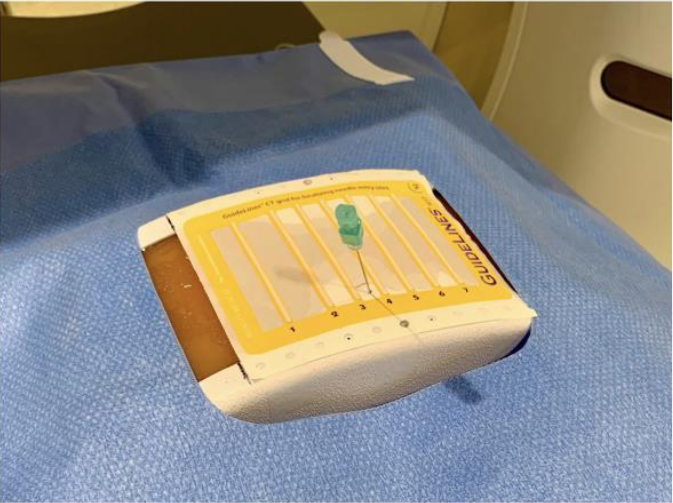
\includegraphics[width=\textwidth]{images/phantom-target.png}
        \caption{Inserimento dell'ago senza AR.}
        \label{fig:figure3c}
    \end{subfigure}
    \begin{subfigure}{0.45\textwidth}
        \centering
        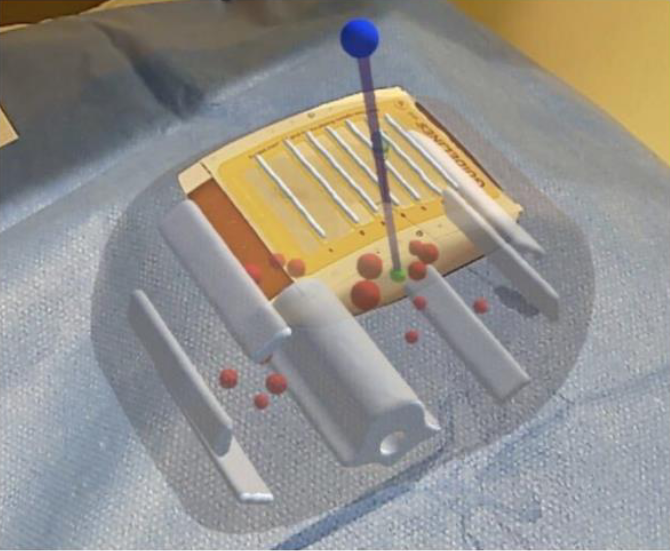
\includegraphics[width=\textwidth]{images/phantom-ologram.png}
        \caption{Inserimento dell'ago con modello tridimensionale e guida dell'ago virtuale proiettati sul fantoccio tramite HoloLens 2.}
        \label{fig:figure3d}
    \end{subfigure}
       \label{fig:figure3}
\end{figure}

Il numero medio totale di passaggi per raggiungere l'obiettivo è stato ridotto da 7,4 passaggi senza AR a 3,4 passaggi con AR (riduzione del 54,2\%).
Il tasso di errore, introdotto nel colpire una lesione non mirata è diminuito dall'11,9\% senza AR (7/59 passaggi con ago) allo 0\% con AR (0/27 passaggi con ago). I passaggi con AR erano più allineati con la traiettoria ideale del bersaglio rispetto a quelli senza AR (offset rispettivamente di 4,6° e 8,0°).

La guida 3D AR può fornire miglioramenti significativi nell'efficienza procedurale e nel risparmio della dose di radiazioni per individuare lesioni difficili e fuori dal piano. La guida AR ha elevato le prestazioni di tutti gli operatori allo stesso livello indipendentemente dalla precedente esperienza clinica.
I risultati chiave dei test effettuati sono i seguenti:
\begin{itemize}
    \item I passaggi totali con ago e la dose di radiazioni sono significativamente ridotti utilizzando la realtà aumentata.
    \item Il tasso di errore, introdotto nel colpire una lesione non mirata viene eliminato utilizzando la realtà aumentata.
    \item La realtà aumentata ha elevato le prestazioni di tutti gli operatori allo stesso livello indipendentemente dalla precedente esperienza clinica.
\end{itemize}

\section{Ambito Educativo}\label{sec:Sezione3.3}

Negli ultimi anni, il settore dell'istruzione ha incorporato nelle classi l'uso di nuove tecnologie e dispositivi informatici, che hanno consentito di implementare nuovi modi per migliorare l'insegnamento e l'apprendimento. La realtà aumentata può essere impiegata per aiutare gli insegnanti a promuovere l'interesse degli studenti nell'apprendimento di determinate materie e concetti astratti in nuove modalità visive. Questo articolo \cite{Augmented-Reality-Teaching-System} propone di sfruttare il potenziale di HoloLens al fine di integrare esperienze AR nelle lezioni e nei laboratori pratici. Nello specifico, viene proposta un'architettura per fornire servizi didattici AR a bassa latenza in un'aula o in un laboratorio. Una latenza così bassa è ottenuta grazie all'uso di dispositivi di edge computing, che esonerano il cloud dalle attività tradizionali richieste dalle applicazioni AR dinamiche (ad esempio, elaborazione dei dati in tempo reale, comunicazioni tra dispositivi AR). A seconda dell'applicazione AR specifica e del numero di utenti, il collegamento wireless (di solito WiFi) potrebbe essere sovraccaricato se la rete non è stata progettata correttamente e le prestazioni complessive dell'applicazione possono essere compromesse, portando a un'elevata latenza e persino a problemi di comunicazione. Per affrontare questo problema, le misurazioni del canale radio e i risultati della simulazione sono stati eseguiti per mezzo di uno strumento di ray-launching 3D sviluppato internamente, che è in grado di modellare e simulare il comportamento di un'aula/laboratorio abilitato per AR in termini di propagazione radio e qualità del servizio.

La Figura \ref{fig:figure32} illustra l'architettura di comunicazione del sistema proposto. In fondo è presente il livello AR-IoT, che è diviso in due sottolivelli: il sottolivello dei dispositivi AR, che è composto dai dispositivi AR utilizzati dagli studenti e dall'insegnante, e il sottolivello dei dispositivi IoT (ovvero, oggetti smart come sensori e attuatori) che sono presenti nell'ambiente. Entrambi i dispositivi AR e IoT sono collegati tramite un punto di accesso WiFi (AP) o un gateway al livello di edge computing, dove vengono eseguiti i servizi educativi AR. Nello specifico, lo strato edge computing è conformato da due sottolivelli:

\begin{itemize}
    \item \textbf{AR Service Sublayer}: utilizza dispositivi di edge computing come cloudlet \footnote{È un data center cloud su piccola scala ottimizzato per la mobilità che si trova ai "margini" di Internet.} o fog di gateway \footnote{È un'architettura che utilizza dispositivi periferici per eseguire una notevole quantità di calcolo, archiviazione e comunicazione localmente per poi instradarla su Internet.} basati su single board computer (SBC) \footnote{È un computer completo costruito su un unico circuito, con microprocessore, memoria, input/output e altre caratteristiche richieste da un computer. } per fornire risposte veloci e distribuite. Gli insegnanti possono agire come amministratori locali dei dispositivi su questo livello per controllare quali contenuti vengono mandati ai dispositivi AR degli studenti. Inoltre, i dispositivi di edge computing di questo livello consentono la condivisione di esperienze AR, potendo così sincronizzare il contenuto condiviso contemporaneamente tra più utenti.
    \item \textbf{AR-IoT Service Sublayer}: consente di interconnettere dispositivi AR e IoT senza soluzione di continuità. Il sistema presentato utilizza Message Queue Telemetry Transport (MQTT) \footnote{È un protocollo di rete leggero di tipo publish-subscribe, che trasporta i messaggi tra i dispositivi. } e un'API (Application Programming Interface) REpresentational State Transfer (REST) per facilitare gli scambi di dati tra più dispositivi eterogenei. Per quanto riguarda il servizio AR-IoT Bridge, si tratta di un componente software che collega le richieste MQTT e API REST, avvalendosi di determinati servizi ausiliari quando necessario.
\end{itemize}

\begin{figure}[t]
    \centering
    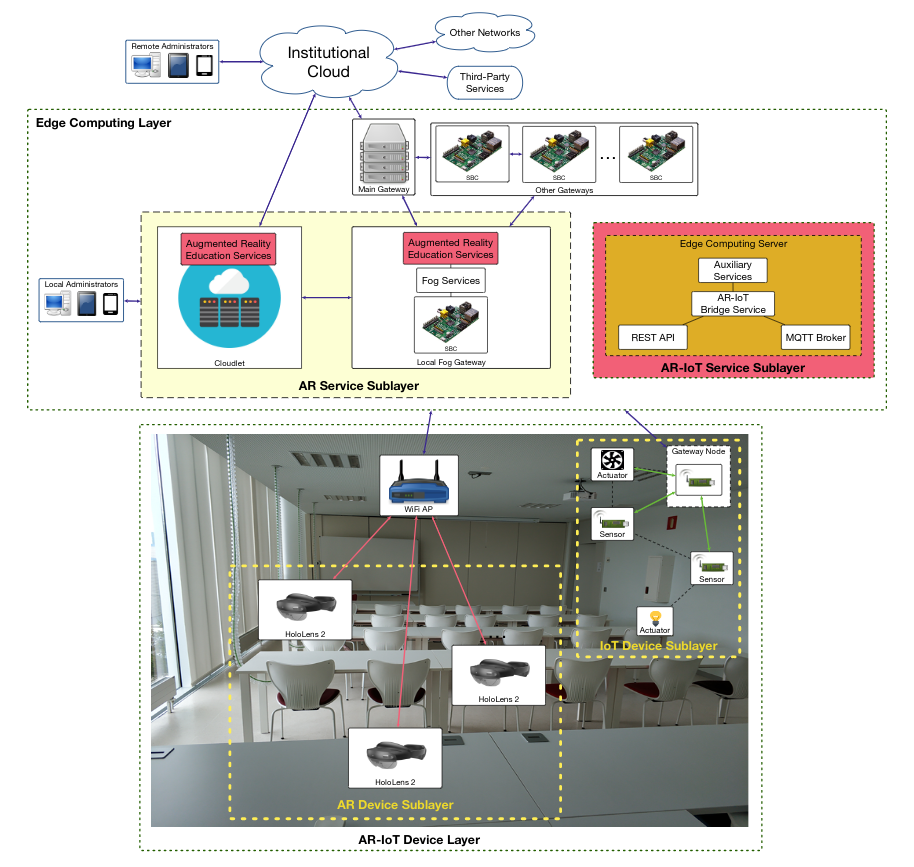
\includegraphics[width=\textwidth]{images/Communications-architecture.png}
    \caption{Architettura di comunicazione del sistema proposto.}
    \label{fig:figure32}
\end{figure}

Entrambi i livelli consentono di implementare le funzionalità più avanzate del sistema:

\begin{itemize}
    \item L'insegnante è in grado di controllare da remoto quando e come il contenuto AR viene visualizzato sui visori HoloLens 2 utilizzati dagli studenti.
    \item Gli studenti possono condividere la stessa esperienza AR e quindi collaborare tra loro per raggiungere un obiettivo comune.
    \item Il sistema sviluppato può interagire con gli oggetti IoT circostanti, consentendo agli utenti AR di ottenere informazioni o di agire con essi.
    \item Poiché l'applicazione HoloLens 2 rileva le azioni eseguite da ogni studente, è possibile registrarle e quindi determinare le prestazioni dello studente o i suoi contributi durante le attività di collaborazione.
\end{itemize}

\section{Ambito Museale}\label{sec:Sezione3.4}
Un altro ambito di applicazione interessante è quello del museo.
Infatti è possibile sviluppare applicazioni AR utili per guidare l'utente all'interno del museo.
Entrando più nello specifico, si può proporre una guida virtuale che, oltre a guidare l'utente, permetta di interagire con i modelli 3D relativi agli artefatti presenti all'interno del museo.
Una soluzione del genere viene proposta in questo articolo \cite{HoloLens-in-museum}, dove è stata utilizzata la prima versione di HoloLens.
Questa procedura mira a creare un quadro di orientamento semplice, interattivo e informativo da utilizzare per gli utenti dei musei. L'applicazione MR richiede all'utente di indossare Microsoft HoloLens ed esplorare una serie di contenuti virtuali attraverso l'interfaccia utente. Un ambiente popolato da reperti museali è necessario per sovrapporre virtualizzazioni digitali e informazioni affinché il sistema di guida virtuale del tour possa funzionare. 
L'applicazione proposta (Figura \ref{fig:figure33}) fornisce le seguenti funzionalità:
\begin{itemize}
    \item Controllo degli ologrammi relativi ai manufatti museali, con possibilità di ruotarli di 360 gradi.
    \item Pulsanti che avviano testo e immagini per permettere all'utente di ricevere informazioni.
    \item Interazione con il sistema di guida virtuale, che presenta informazioni audio e video in tempo reale.
    \item Utilizzo di piccoli cerchi che funzionano come oggetti trigger per rivelare informazioni su particolari aree di interesse.
\end{itemize}

\begin{figure}[t]
    \centering
    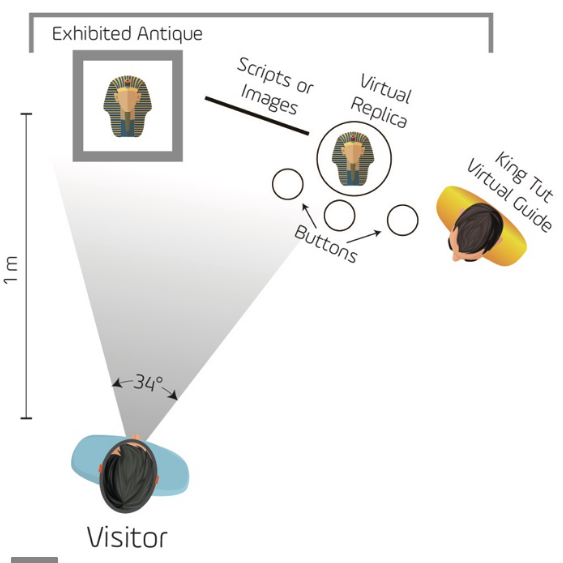
\includegraphics[width=0.6\textwidth]{images/museum.png}
    \caption{Scena di esempio dell'applicazione.}
    \label{fig:figure33}
\end{figure}

Nell'articolo vengono presentati i risultati dei test eseguiti su un campione di utenti.
Il campione di popolazione valutato includeva nove esperti in diverse discipline accademiche che vanno dall'interazione uomo-macchina (in inglese human-computer interaction, HCI) alla comunicazione visiva. Considerando gli esperti di HCI e di comunicazione visiva in questa valutazione è stata presa in considerazione la loro capacità di valutare l'usabilità, l'interattività e il livello di esperienza utente acquisita. Quindi, gli esperti di studi museali sono stati considerati per valutare se questo sistema può raggiungere ciò che i visitatori richiedono nei musei e per strutturarlo in base alla natura delle visite. Considerare gli esperti per questa valutazione ha un doppio vantaggio: come menzionato hanno esperienza e possono anche essere generalmente visitatori di musei, quindi le loro risposte possono essere più critiche e vantaggiose per lo studio rispetto a quelle  dei normali visitatori del museo.

Il prototipo dell'applicazione ha ottenuto risultati complessivamente positivi sia in termini di usabilità che di accessibilità.